\chapter{Rendering Mode 0}
Wie oben bereits erwähnt, handelt es sich bei dem Modus 0 um eine Einstellung des \ac{GBA}, welche 4 reguläre Hintergründe anzeigen kann. Reguläre Hintergründe sind weder skalierbar, noch rotierbar. Das ist der Unterschied zu den affinen Hintergründen. Angezeigt werden die verschiedenen Karten anhand der eingestellten Priorität, wobei die niedrigste Nummer der höchsten Priorität entspricht. Die unterschiedlichen Hintergünde können entweder sogenannte Tilemaps sein, welche sich aus Kacheln zusammensetzen, oder Sprites, also Objekte oder Bilder. Zuerst wird auf die Tilemaps und Kacheln genauer eingegangen. \citep{mode}
\section{Tilemaps}
\begin{wrapfigure}{R}{0mm}
	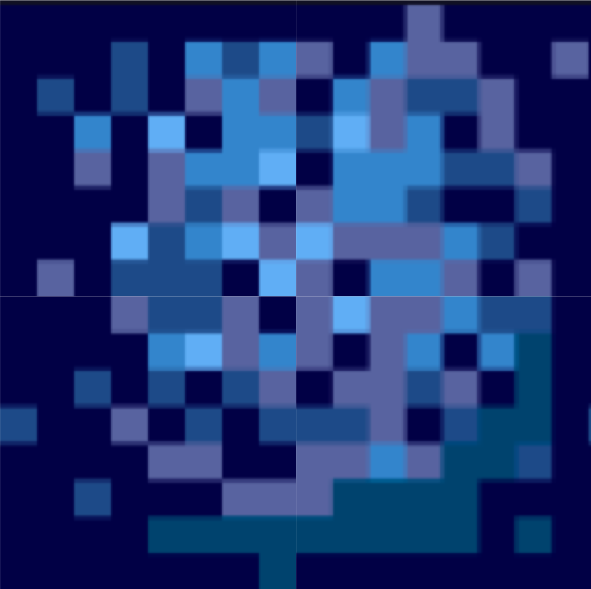
\includegraphics[height=40mm]{img/tile_blue.png}
	\caption{Beispieltile}
	\label{example_tile}
\end{wrapfigure}
Jede Kachel besteht standardmäßig aus 16x16 Pixel. Diese Zusammensetzung aus Pixeln wird in einem Array aus Hexadezimalen, dem Tileset, gespeichert. So wird in einem externen Dokument in zwei Schritten der Hintergrund aufgebaut. Zuerst werden die Pixel der Reihe nach in dem Tileset gespeichert. Danach wird der Hintergrund aus den vorher angelegten Blöcken zusammengesetzt. Es entsteht eine Matrix, die sogenannte Tilemap. 

Die Blöcke werden allerdings nicht als 16x16 Pixel große Bitfolgen abgespeichert, sondern nochmal aufgeteilt in vier 8x8 Pixel große Objekte. Das hat den Vorteil, dass diese Bauteile meist wiederverwendbar sind, und so nochmal Speicherplatz gespart wird. Das kann zum Beispiel der Fall sein, wenn eine Kachel nur aus einem Farbton besteht. Dann muss nur ein einziger 8x8 Baustein abgespeichert werden und kann vier mal eingesetzt werden. Die Zusammensetzung eines Blockes wird im Folgenden an anhand des Beispiels in Abbildung \ref{tile_quarter} dargestellt.
\begin{figure}[H]
	\centering
	\begin{subfigure}{.5\textwidth}
		\centering
		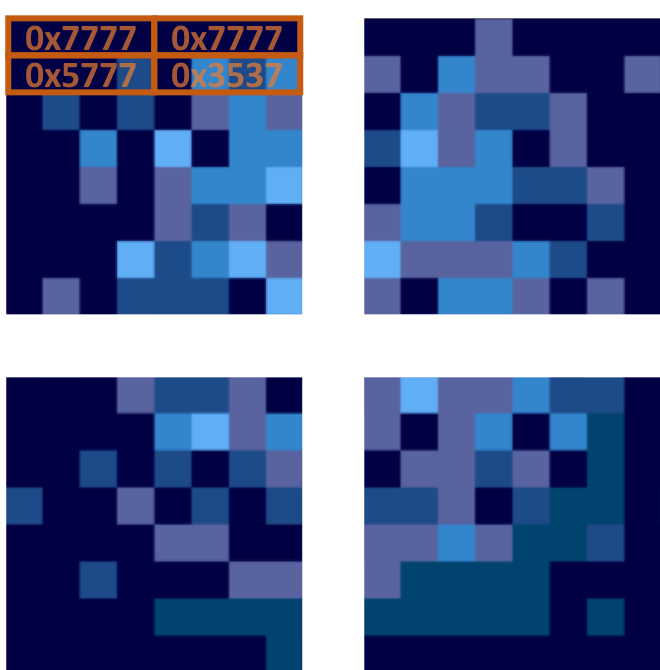
\includegraphics[height=40mm]{img/tile_pixels.png}
		\caption{Pixelabfolge der einzelnen Bestandteile}
	\end{subfigure}%
	\begin{subfigure}{.5\textwidth}
		\centering
		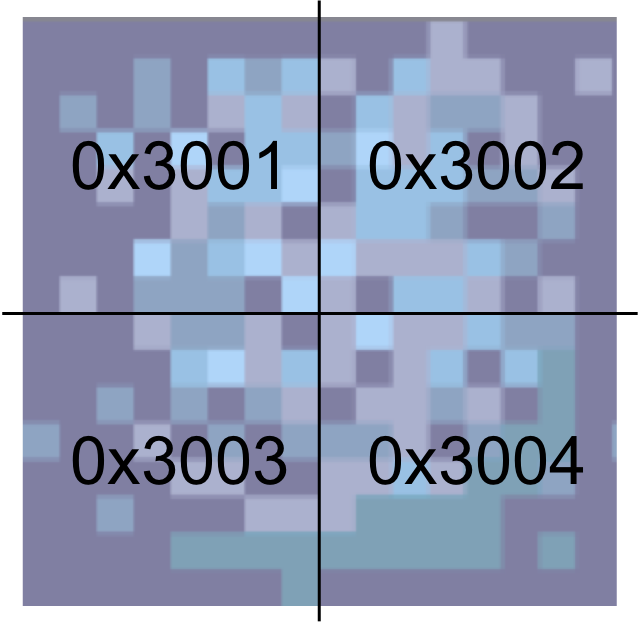
\includegraphics[height=40mm]{img/tile_blue_quarter.png}
		\caption{Aufteilung eines Tiles in vier 8x8 Pixel Blöcke}
	\end{subfigure}
	\caption[Bestandteile eines Blocks]{}
	\label{tile_quarter}
\end{figure}
Jedes Pixel wird als eine Stelle in der Hexadezimalen, also in 4 Bit, abgespeichert. Die Reihenfolge der Pixel erfolgt Zeilenweise, genauso wie die Abfolge der Kacheln selbst. So kann ein Block in der Tilemap nicht einfach der Reihe nach referenziert werden, sondern die obere Hälfte muss in der ersten Zeile abgerufen werden, die untere in der darauf folgenden. Außerdem enthält ein Screenblock bei dem \ac{GBA} noch zusätzliche Informationen, welche in Tabelle \ref{tile_memory} dargestellt sind.
\begin{table}[H]
\centering
\begin{tabular}{|p{1cm}|p{1cm}|p{4cm}|p{9cm}|}
\hline
\textbf{Bits} & \textbf{Name} & \textbf{Definition} & \textbf{Beschreibung} \\ \hline
0 - 9 & TID & SE\_ID\# & Blockindex des Screen-entries (SE) \\ \hline
A - B & HF, VF & SE\_HFLIP, SE\_VFLIP. SE\_FLIP\# & Horizontale bzw. Vertikale Spiegelung \\ \hline
C - F & PB & SE\_PALBANK\# & Palette welche im 16-Farben Modus benutzt wird. Hat keinen Effekt für 256-Farben Hintergründe. \\ \hline
\end{tabular}
\caption{Einstellungen eines Blockes \citep{tile}}
\label{tile_memory}
\end{table}

\begin{wrapfigure}{L}{0mm}
	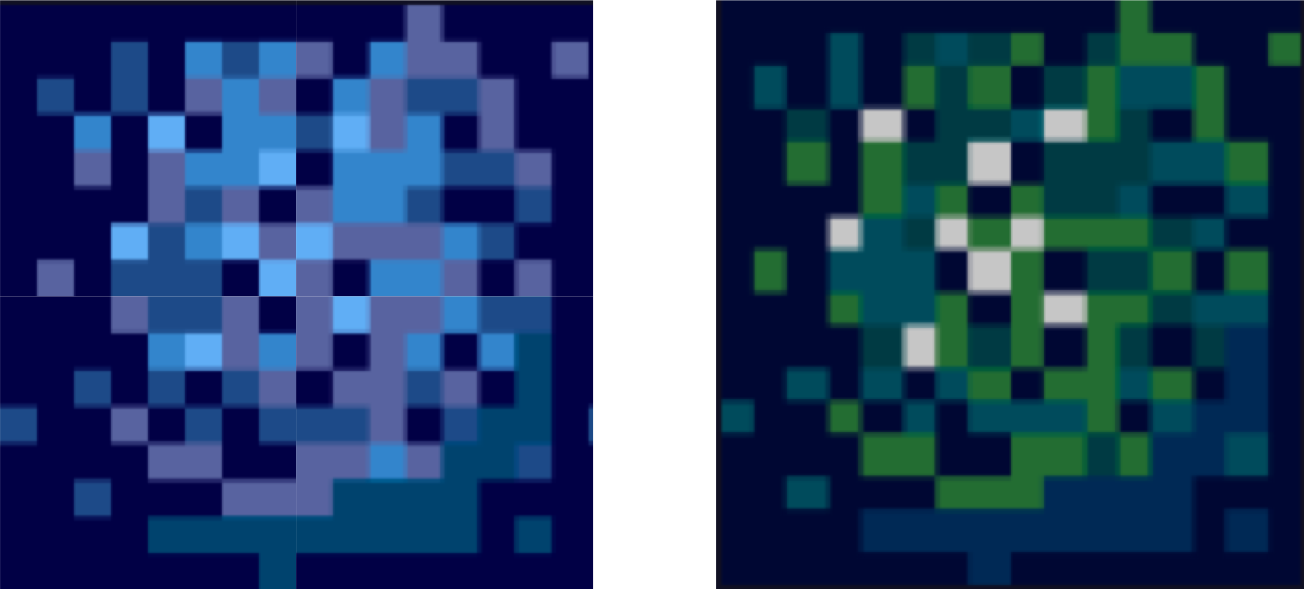
\includegraphics[height=30mm]{img/tiles_palette.png}
	\caption{Anwendung verschiedener Paletten}
	\label{tile_palettes}
	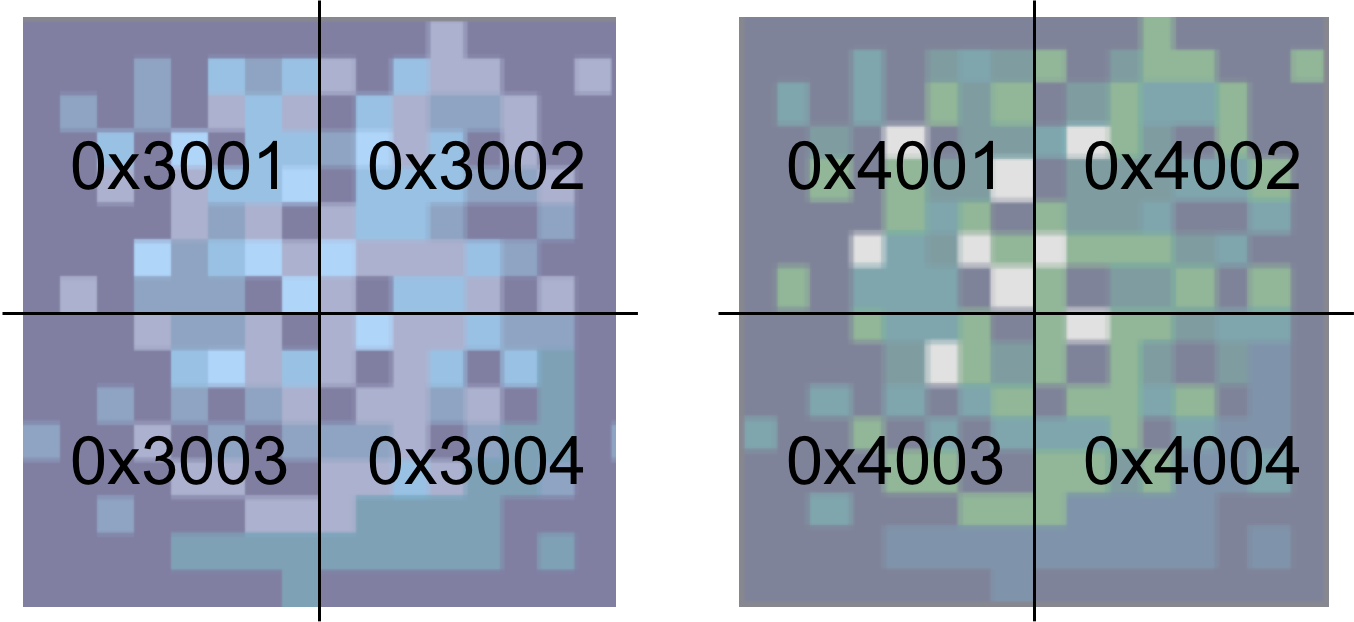
\includegraphics[height=30mm]{img/tiles_palette_quarter.png}
	\caption{Hex-Codes der Paletten}
	\label{tile_palettes_hex}
\end{wrapfigure}
Um diese Zusammensetzung beispielhaft darzustellen, kann man auf den Blöcken links in den Abb. \ref{tile_palettes} und \ref{tile_palettes_hex} die Verwendung verschiedener Paletten sehen. 

Die Palette wird ebenfalls extern angelegt und im Screenblock, entsprechend der oberen Tabelle, referenziert. Eine Palette wird nur bei einer Bittiefe von 4 (16 Farben, 16 Unterpaletten) angelegt, nicht aber bei 8 (256 Farben / 1 Palette), die entsprechenden Bits werden dann auf 0 gesetzt. 

Im \textbf{\ac{VRAM}} ist Platz für 32 Screenblocks um die Tilemaps zu speichern. Durch die Länge eines jeden Screenblocks ergibt sich, dass insgesamt 32x32 \ac{SE} hineinpassen. Das heißt, es kann maximal eine 256x256 Pixel große Karte gespeichert werden. \citep{gbatek} Die größeren Karten verwenden einfach mehr als einen Screenblock. Der in \textbf{REG\_BGxCNT} gesetzte \ac{SE}-Index ist der Bildschirmbasisblock, der den Beginn der Tilemap angibt. Größere Hintergründe verwenden nicht einfach mehrere Bildschirmblöcke, sondern sie werden als vier separate Karten aufgerufen. Jeder nummerierte Block ist ein Kontingentblock im Speicher. Dies bedeutet, um den \ac{SE}-Index zu erhalten, braucht man zuerst den Screenblock, in dem man sich befindet und dann die \ac{SE}-Nummer in diesem Screenblock. \citep{tile}

Die Zusammensetzung der einzelnen Screenblock-Layouts erfolgt wiederum der Reihe nach. Im Programm selbst wiederholen sich die jeweiligen Screenblocks immer wieder, sodass ein unendlich großer Hintergrund simuliert wird und die "Spiel-Welt" sozusagen nie zu Ende ist. Die unten aufgeführte Karte in Abb. \ref{tilemap} ist aus zwei Screenblocks in einem 64x32 Layout dargestellt. Der Code darunter veranschaulicht das Laden der einzelnen Komponenten in das Spiel. Hier werden zunächste die einzelnen Komponenten, wie die Palette, die Kacheln und die Tilemap in den \textbf{\ac{VRAM}} geladen und in \textbf{REG\_BG0CNT} zu einem Hintergrundobjekt zusammengeführt. Danach wird der Rendering Mode, in diesem Fall mit \textbf{DCNT\_MODE0} auf 0 gesetzt. Die while-Schleife im Anschluss ermöglicht das unbegrenzte scrollen durch den Bildschirm mit den Pfeiltasten.
\begin{figure}[h]
	\centering
	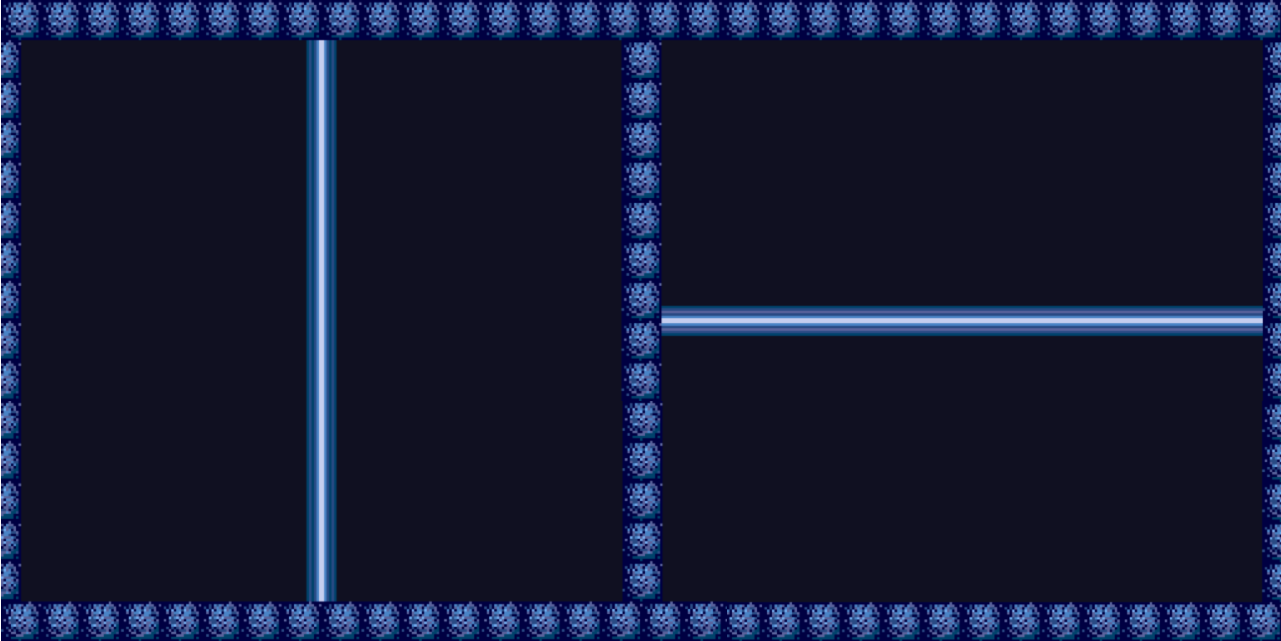
\includegraphics[height=70mm]{img/tilemap.png}
	\caption{Beispiel einer 64 x 32 Tilemap}
	\label{tilemap}
\end{figure}

\lstinputlisting[language=C, frame=single, breaklines = true, numbers=left, basicstyle=\ttfamily, keywordstyle=\color{blue}\ttfamily, stringstyle=\color{red}\ttfamily, commentstyle=\color{green}\ttfamily, label=tilemap_code,caption=main() Funktion]{code/tilemap.c}
\section{Sprites}
\begin{wrapfigure}{R}{0mm}
	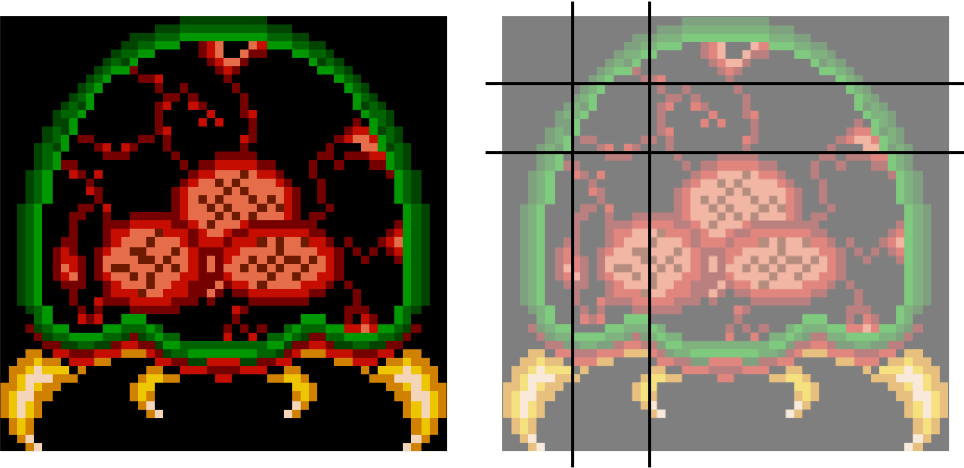
\includegraphics[height=40mm]{img/sprites.png}
	\caption{Beispiel Sprite und Aufteilung in einzelne Kacheln}
	\label{sprites}
\end{wrapfigure}
Unter Sprites versteht man grundsätzlich Hintergrundbilder. Meist werden sie als Dekoration in den Hintergrund eingebettet, da sie nicht das komplette Display einnehmen und so an beliebigen Stellen eingefügt werden können. Die Sprites sind wiederum als eine Zusammensetzung aus 8x8 Pixel großen Bausteinen gespeichert, wie Kacheln. Das ist in Abbildung \ref{sprites} beispielhaft dargestellt.

Der Hauptunterschied zwischen Kacheln (Tiles) und Sprites liegt darin, dass die Tilemap den gesamten Hintergrund bedeckt. Das heißt, an jeder Stelle des Hintergrundes wird ein Pixel bzw. Ein Block abgespeichert. Dagegen ist ein Sprite eine eigene Zusammensetzung aus Blöcken, die an einer festen Stelle im Hintergrund angezeigt wird. 

Die Spezifikationen eines Sprites werden in dem sogenannten \textbf{\ac{OAM}} gespeichert. Dieser besteht aus zwei Strukturen: Der \textbf{OBJ\_ATTR}-Struktur, welche alle regulären Attribute enthält, und der \textbf{OBJ\_AFFINE}-Struktur, welche potentielle Transformationen enthält.
Die \textbf{OBJ\_ATTR}-Struktur besteht aus drei 16-Bit-Attributen für Eigenschaften wie Größe, Form, Grundblock etc. Diese drei Attribute sind im Folgenden genauer erläutert.
\paragraph{Attribut 0}
%\subsection{Attribut 0}
Das erste Attribut enthält einige Informationen, aber die wichtigsten Bestandteile hier sind die y-Koordinate und die Form des Sprites. Wichtig ist auch, ob das Sprite transformierbar ist (ein affines Sprite) und ob die Kacheln eine Bittiefe von 4 (16 Farben, 16 Unterpaletten) oder 8 (256 Farben / 1 Palette) haben.
%\begin{table}[ht]
%\centering
%\begin{tabular}{|p{1cm}|p{1cm}|p{3.5cm}|p{9cm}|}
%\hline
%\textbf{Bits} & \textbf{Name} & \textbf{Definition} & \textbf{Beschreibung} \\ \hline
%0 - 7 & Y & ATTR0\_Y\# & Y-Koordinate (Position des Sprites) \\ \hline
%8 - 9 & OM & ATTR0\_REG, ATTR0\_AFF, ATTR0\_HIDE, ATTR0\_AFF\_DBL. ATTR0\_MODE\# & Modus des Sprites: 
%{\begin{itemize}
%	\setlength\itemsep{0em}
%	\item 00: Normale Anzeige
%	\item 01: Affine Anzeige - Matrix wird in Attr. 1 angegeben
%	\item 10: Keine Anzeige (versteckt)
%	\item 11: Affine Doppelanzeige
%\end{itemize}} \\ \hline
%A - B & GM & ATTR0\_BLEND, ATTR0\_WIN. ATTR0\_GFX\# & Spezialeffekte:
%{\begin{itemize}
%	\setlength\itemsep{0em}
%	\item00: Normale Anzeige
%	\item01: Alpha Blending
%	\item10: Keine Anzeige, aber ist Teil des Bildschirms
%	\item11: Verboten
%\end{itemize}} \\ \hline
%C & Mos & ATTR0\_MOSAIC & Mosaik Effekt \\ \hline
%D & CM & ATTR0\_4BPP, ATTR0\_8BPP & Farbauswahl \\ \hline
%E - F & Sh & ATTR0\_SQUARE, ATTR0\_WIDE, ATTR0\_TALL. ATTR0\_SHAPE\# & Form des Sprites \\ \hline
%\end{tabular}
%\caption{Zusammensetzung von Attribut 0 eines Sprites}
%\label{sprite-attr0}
%\end{table}
\paragraph{Attribut 1}
%\subsection{Attribut 1}
Die wichtigsten Bestandteile dieses Attributs sind die X-Koordinate und die Größe des Sprites. Die Rolle der Bits 8 bis 14 hängt davon ab, ob dies ein affiner Sprite ist. Wenn dies der Fall ist, geben diese Bits an, welcher der 32 OBJ\_AFFINE verwendet werden soll. Wenn nicht, enthalten sie sogenannte flipping flags, welche eine horizontale bzw. vertikale Spiegelung des Sprites zur Folge haben.
%\begin{table}[ht]
%\centering
%\begin{tabular}{|p{1cm}|p{1cm}|p{3.5cm}|p{9cm}|}
%\hline
%\textbf{Bits} & \textbf{Name} & \textbf{Definition} & \textbf{Beschreibung} \\ \hline
%0 - 8 & X & ATTR1\_Y\# & X-Koordinate (Position des Sprites) \\ \hline
%9 - D & AID & ATTR1\_AFF & Affiner Index, nur gültig falls Affine Flag in Attribut 0 gesetzt ist \\ \hline
%C - D & HF, VF & ATTR1\_HFLIP, ATTR1\_VFLIP. ATTR1\_FLIP\# & Horizontale bzw. Vertikale Spiegelung, nur gültig falls Affine Flag in Attribut 0 nicht gesetzt ist \\ \hline
%E - F & Sz & ATTR1\_SIZE & Größe des Sprites \\ \hline
%\end{tabular}
%\caption{Zusammensetzung von Attribut 1 eines Sprites}
%\label{sprite-attr1}
%\end{table}
\paragraph{Attribut 2} 
%\subsection{Attribut 2}
Dieses Attribut enthält Informationen darüber, welche Kacheln angezeigt und welche Priorität diese bezogen auf die Hintergründe haben. Falls dies ein 4bpp-Sprite ist, wird hier auch die Farbpalette angegeben. \citep{sprites}
%\begin{table}[ht]
%\centering
%\begin{tabular}{|p{1cm}|p{1cm}|p{3.5cm}|p{9cm}|}
%\hline
%\textbf{Bits} & \textbf{Name} & \textbf{Definition} & \textbf{Beschreibung} \\ \hline
%0 - 9 & TID & ATTR2\_ID\# & Index des Basisblocks \\ \hline
%A - B & Pr & ATTR1\_PRIO\# & Anzeigepriorität \\ \hline
%C - F & PB & ATTR1\_PALBANK\# & Palette für 16-Farbmodus \\ \hline
%\end{tabular}
%\caption{Zusammensetzung von Attribut 2 eines Sprites}
%\label{sprite-attr2}
%\end{table}

Die Initialisierung eines Sprites wird anhand eines kurzen Code-Ausschnitts in Listing \ref{init_sprite} erläutert. Hier werden zuerst der Index der ersten Kachel und die Palette zwischengespeichert. Dann werden der Reihe nach alle drei Attribute so gesetzt, dass nur die wichtigsten Bestandteile verändert werden müssen, die restlichen Bits bleiben demnach 0. In der main()-Funktion wird anschließend wieder der Hintergrund initialisiert, ähnlich wie in Listing \ref{tilemap_code}.
\lstinputlisting[language=C, frame=single, breaklines = true, numbers=left, basicstyle=\ttfamily, keywordstyle=\color{blue}\ttfamily, stringstyle=\color{red}\ttfamily, commentstyle=\color{green}\ttfamily, label=init_sprite,caption=Sprite Initialisierung]{code/init_sprite.c}


